\chapter{Code listings}\label{app:code}
\begin{figure}[hbtp]
    \centering
    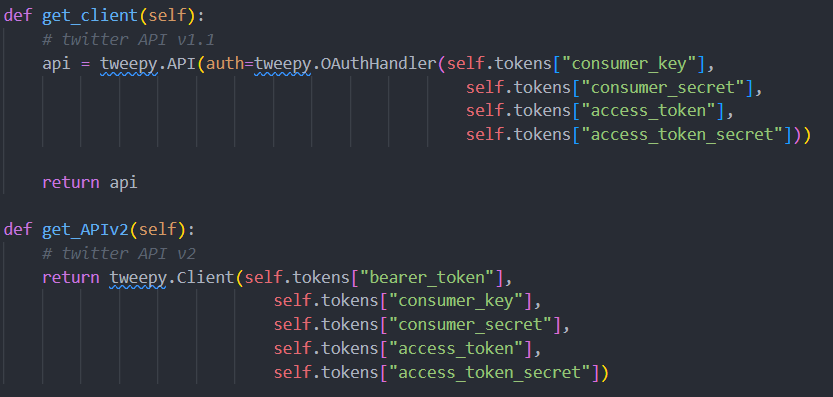
\includegraphics[width=0.6\textwidth]{../images/setup-api-conn.png}
    \caption{Code used to connect to twitter API}
    \label{fig:tweepy-conn}
\end{figure}
\begin{figure}[hbtp]
    \centering
    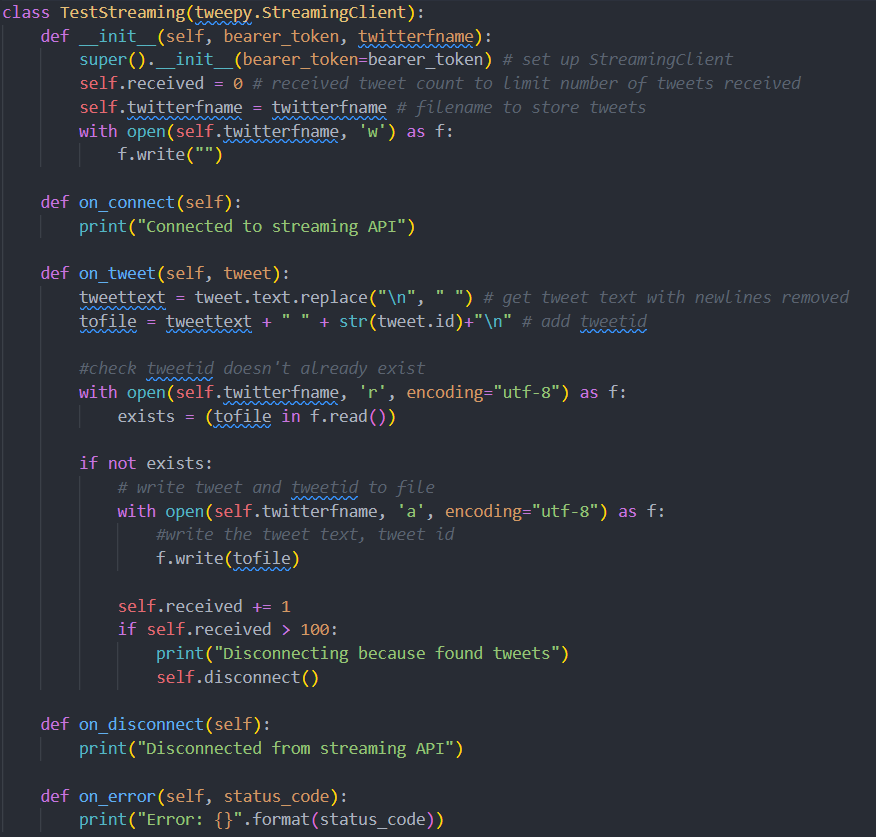
\includegraphics[width=0.6\textwidth]{../images/streamingclient.png}
    \caption{Use of StreamingClient to collect live twitter data}
    \label{fig:live-data}
\end{figure}
\begin{figure}[hbtp]
    \centering
    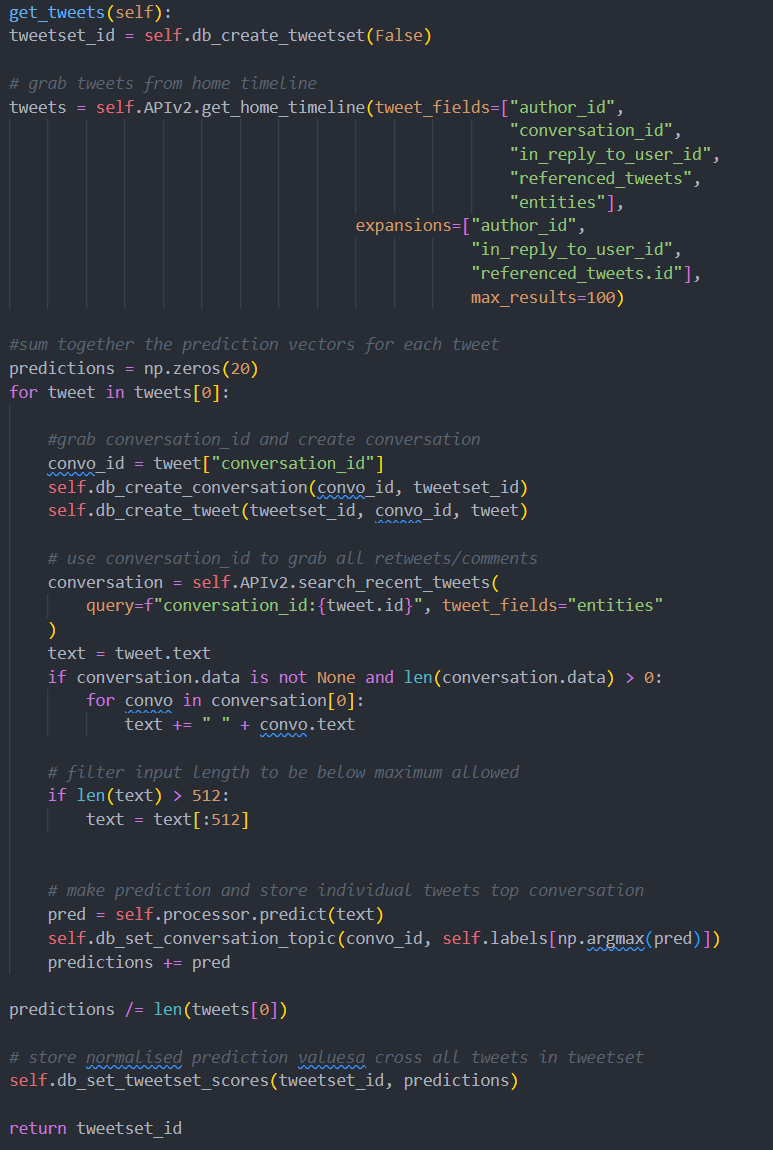
\includegraphics[width=0.6\textwidth]{../images/get_home_timeline.png}
    \caption{Use of API connections to get users home timeline}
    \label{fig:user-data}
\end{figure}